\documentclass[11pt,a4paper]{article}

% --- Packages ---
\usepackage[utf8]{inputenc}
\usepackage[margin=1in]{geometry}
\usepackage{amsmath,amssymb,amsfonts,amsthm}
\usepackage{booktabs}
\usepackage{tabularx}
\usepackage{graphicx}
\usepackage{xcolor}
\usepackage{hyperref}
\usepackage{cite}
\usepackage{listings}
\usepackage{tikz}
\usetikzlibrary{shapes,arrows,positioning,calc,fit}
\usepackage{tcolorbox}
\usepackage{microtype}
\usepackage{fancyhdr}
\usepackage{enumitem}

% --- Hyperref Setup ---
\hypersetup{
    colorlinks=true,
    linkcolor=blue!70!black,
    citecolor=red!70!black,
    urlcolor=blue!80!black,
    pdftitle={The Virtual Private Phone (VPP): Decoupled Physical Architecture for Anti-Forensic Mobile Security and Resilient Digital Identity},
    pdfauthor={Ali Ganji},
    pdfkeywords={Mobile Forensics, Anti-Forensics, Decoupled Architecture, Thin-Client, Hardware Separation, Remote Attestation, Ephemeral OS}
}

% --- Header and Footer ---
\pagestyle{fancy}
\fancyhf{}
\rhead{\textit{The Virtual Private Phone (VPP)}}
\lhead{Ali Ganji \textbullet\ LabXIII}
\cfoot{\thepage}

% --- Custom Environments ---
\newtheorem{definition}{Definition}
\newtheorem{theorem}{Theorem}
\newtheorem{property}{Property}

\definecolor{codegreen}{rgb}{0,0.6,0}
\definecolor{codegray}{rgb}{0.5,0.5,0.5}
\definecolor{codepurple}{rgb}{0.58,0,0.82}
\definecolor{backcolour}{rgb}{0.96,0.96,0.96}

\lstdefinestyle{mystyle}{
    backgroundcolor=\color{backcolour},   
    commentstyle=\color{codegreen},
    keywordstyle=\color{magenta},
    numberstyle=\tiny\color{codegray},
    stringstyle=\color{codepurple},
    basicstyle=\ttfamily\footnotesize,
    breakatwhitespace=false,         
    breaklines=true,                 
    captionpos=b,                    
    keepspaces=true,                 
    numbers=left,                    
    numbersep=5pt,                  
    showspaces=false,                
    showstringspaces=false,
    showtabs=false,                  
    tabsize=2
}
\lstset{style=mystyle}

% --- Title and Metadata ---
\title{\textbf{The Virtual Private Phone (VPP):\\Decoupled Physical Architecture for Anti-Forensic Mobile Security and Resilient Digital Identity}\\[0.5em]\large An Architectural \& Research Proposal}

\author{
    \textbf{Ali Ganji}\\
    \textit{Principal Security Researcher}\\
    LabXIII Research\\
    \url{https://xiii.me} \quad \textbullet \quad \texttt{aliganji@labxiii.org}
}

\date{\today}

\begin{document}

\maketitle

\begin{abstract}
Imagine for a moment that you are a hacker, an investigative researcher, or an enterprising criminal whose recent activities have attracted the undivided attention of law enforcement. The blue lights flash, the handcuffs click, and your phone—the intimate little black box holding your entire existence, your client notes, your financial secrets, and a camera roll that could easily fill six dramatic seasons of a Netflix true-crime documentary—is sitting on a police evidence desk marked as ``Exhibit~A''. 

Now consider the fundamental injustice of this moment: regardless of alleged guilt or innocence, it is completely unfair to human data privacy that grabbing a 200-gram slab of glass from your pocket grants investigators an all-access VIP backstage pass to dig, dive, and forensically excavate every corner of your digital life. Why should one fragile piece of hardware hold our private memories, act as our legal identity, and then betray us the exact millisecond it is snatched from our hands? Your lawyer can handle the screenplay; we decided to fix the phone.

In this research proposal, we present the \textbf{Virtual Private Phone (VPP)}: \textit{One phone stays home. The other goes in your pocket.} The VPP physically bifurcates the smartphone into two distinct machines: an untrusted, disposable, RAM-only \textit{Frontend Handset} that you carry into the world, and a secure \textit{Backend Core} safely plugged into the wall in your domestic sanctuary. The pocket handset contains zero persistent flash storage, zero application databases, and zero encryption keys—it is merely an ephemeral, low-latency streaming window and remote sensor controller. If the police seize your pocket phone—whether you refuse the password, surrender the PIN under duress, or have your thumb held against the biometric sensor—they find absolutely nothing. The moment you dial an emergency out-of-band hotline or the device is sealed in a Faraday bag, the backend severs the session, and the pocket handset's volatile memory is zeroized in under 50 milliseconds. The police are left holding a dead piece of glass, your digital environment remains safely running at home, and the operational mandate is fulfilled: \textit{to lose physical possession of the handset without losing control of the phone.}
\end{abstract}

\vspace{1em}
\noindent\textbf{Keywords:} Mobile Security, Digital Forensics, Anti-Forensics, Decoupled Architecture, Hardware Abstraction Virtualization, Cryptographic Revocation, Remote Attestation, Ephemeral Systems.

\newpage
\tableofcontents
\newpage

\section{Introduction}
\label{sec:introduction}

The modern smartphone represents the most intimate, comprehensive, and high-value intelligence repository ever created. It is simultaneously an authentication token, a biometric scanner, a personal vault of encrypted communications, a real-time tracking beacon, and an archive of photographic and textual metadata. Yet, by historical artifact of engineering design, society mandates that this comprehensive data repository must travel everywhere with its owner, physically exposed in pockets, bags, vehicle mounts, and hands.

\subsection{The Monolithic Vulnerability}
The fundamental security flaw of contemporary mobile computing is its \textit{monolithic physical coupling}: the computational brain, the cryptographic keys, the persistent storage, and the physical human-computer interaction (HCI) sensors are bound within a single 200-gram slab of glass, silicon, and aluminum. 

This coupling precipitates severe security failures:
\begin{enumerate}[label=(\roman*)]
    \item \textbf{Physical Custody and Involuntary Surrender:} In scenarios involving targeted theft, customs/border inspections, or law enforcement detention, physical control of the device passes instantly from the legitimate operator to an adversarial party. If the device is seized in an After First Unlock (AFU) state—or if the operator is coerced into providing a PIN or biometric unlock—the entire digital identity is compromised.
    \item \textbf{The Inadequacy of Remote Wipe:} Traditional defenses rely on Over-the-Air (OTA) remote wiping services (e.g., Apple Find My, Google Find My Device, enterprise MDM protocols). However, these mechanisms suffer from an unresolvable race condition: the moment a device is placed into a radio-frequency (RF) shielding enclosure (a Faraday bag) or has its SIM card ejected, the device is permanently severed from the wiping command while remaining fully vulnerable to local hardware-based extraction techniques~\cite{casey2011digital, nist800101r1}.
    \item \textbf{Identity Destruction upon Device Loss:} Conversely, when a security-conscious user loses an ordinary phone on public transit, the disruption is catastrophic. Two-factor authentication (2FA) SMS codes and push notifications are routed to the lost device; cryptographic keys are trapped inside it; and restoring the environment requires hours or days of high-risk recovery ceremonies.
\end{enumerate}

\subsection{The Operational Scenarios}
To ground the practical urgency of this paradigm shift, we evaluate two operational scenarios reflecting realistic adversarial engagements.

\subsubsection{Scenario A: Law Enforcement Confiscation Under AFU}
Consider an operator who is detained by law enforcement while their device is active and unlocked on a table displaying an active messaging inbox. The handset is immediately confiscated. In an ordinary system, an examiner holding the unlocked handset can freely browse historical records, download unencrypted local databases, and image the flash storage before any timeout occurs. 

In the model proposed in this paper, the operator utilizes a secondary, out-of-band communication channel (e.g., an authenticated telephone hotline, an emergency IVR, or a pre-shared duress signal) to initiate an instantaneous revocation. The backend server severs the active transport pipeline, invalidates cryptographic session keys, and commands the client to zeroize all ephemeral volatile memory. While an examiner may have viewed what was rendered on the screen at the exact second of seizure, any subsequent screen interaction fails, zero stored databases exist on the handset, and no cryptographic pathway remains to reconnect to the user's data vault.

\subsubsection{Scenario B: Pre-emptive Isolation for High-Risk Operators}
Consider a cybersecurity researcher or investigative journalist traveling to high-risk environments or academic security conferences. The researcher frequently carries sensitive exploit code, client vulnerability disclosures, and proprietary notes. In standard operational tradecraft, the researcher is forced to "burn" their daily phone, carrying an inconvenient, feature-stripped "burner" phone, thereby losing access to their primary telephone number, registered apps, and development environments.

Under our proposed architecture, the researcher decides \textit{in advance} where their operating environment lives. The entire execution environment, primary SIM, and persistent records remain hosted securely at home. If the portable handset is dropped, stolen, or searched at a transit checkpoint, the operator simply revokes the device pairing, procures an off-the-shelf replacement handset, authenticates, and resumes the session within minutes without needing to rebuild their operating environment from scratch.

\subsection{Research Contributions and Proposal Scope}
In this research proposal, we present the architectural specification, formal threat model, and experimental verification roadmap for the \textbf{Virtual Private Phone (VPP)}. Our core contributions include:
\begin{itemize}
    \item \textbf{Bifurcated Thin-Client Architecture:} We propose a physical and logical decoupling of the smartphone into an untrusted, stateless \textit{Frontend Handset} and a secure, stationary \textit{Backend Core}.
    \item \textbf{Virtual Hardware Abstraction Layer (V-HAL) Specification:} We design a bidirectional peripheral virtualization pipeline that forwards multi-touch, microphone, camera, and sensor data with an engineering latency budget under 40\,ms, allowing the remote backend to behave as a seamless, local device.
    \item \textbf{Deterministic Ephemeral Anti-Forensics:} We specify an ephemeral, RAM-only frontend operating system design that maintains zero persistent storage of application databases, media files, or long-term credentials, preventing physical extraction by commercial forensic suites.
    \item \textbf{Out-of-Band Revocation Protocol:} We formalize a zero-knowledge, cryptographically enforced revocation protocol that terminates active sessions and commands client memory zeroization within milliseconds of an out-of-band trigger.
    \item \textbf{Verification Methodology and Testbed Framework:} We define the concrete experimental testbed and empirical verification protocols (including the Two-Handset Table Protocol and the Outdoor Mobility Protocol) required to validate the system prior to practical deployment.
\end{itemize}

\section{Background and Related Work}
\label{sec:background}

Understanding the security imperatives of the Virtual Private Phone requires an examination of modern digital forensics methodologies, cryptographic key state transitions in mobile operating systems, and the limitations of current remote computing paradigms.

\subsection{Mobile Device Forensics and Acquisition Modalities}
Mobile forensics follows established international standards such as ISO/IEC 27037~\cite{iso27037} and NIST SP 800-101 Revision 1~\cite{nist800101r1}. Forensic acquisition of mobile hardware broadly falls into three distinct tiers:
\begin{enumerate}
    \item \textbf{Logical Acquisition:} Involves communicating via standard operating system APIs (e.g., Android Debug Bridge or Apple iTunes backup protocols) to export user-accessible file systems, application containers, call logs, and SMS databases.
    \item \textbf{File System Acquisition:} Involves exploiting system-level privileges or bootloader vulnerabilities to extract the raw partition structure, including sandbox-isolated directories, hidden app stores, and unallocated space.
    \item \textbf{Physical Acquisition:} Involves a bit-by-bit physical clone of the underlying non-volatile flash storage (NAND / UFS / NVMe). This can be achieved through specialized hardware exploitation tools (e.g., Cellebrite UFED, Magnet GrayKey), JTAG testing interfaces, or physical chip-off extraction.
\end{enumerate}

\subsection{The Cryptographic State Problem: BFU vs. AFU}
Modern mobile operating systems utilize sophisticated File-Based Encryption (FBE) architectures backed by dedicated hardware security modules (Apple Secure Enclave Processor (SEP), Google Titan M2)~\cite{grapheneos2024}. The vulnerability profile of a device depends fundamentally on its operational state:
\begin{itemize}
    \item \textbf{Before First Unlock (BFU):} Following a system reboot, the cryptographic Master Key ($K_{master}$) and user-credential derived keys ($K_{user}$) are absent from dynamic volatile RAM. The device is in a secure, encrypted state. Forensic extraction of plaintext databases without knowledge of the passcode is mathematically infeasible within standard time bounds.
    \item \textbf{After First Unlock (AFU):} Once the user enters their PIN, password, or biometric credential for the first time following a boot cycle, $K_{user}$ is derived by the hardware security coprocessor and cached in volatile RAM to facilitate background task processing, notification receipt, and seamless unlocking. 
\end{itemize}

In the AFU state, even if the screen is subsequently locked, the class-level cryptographic keys protecting local SQLite databases (e.g., Signal messaging databases, WhatsApp chat histories, browser caches) remain resident in main memory. Specialized forensic toolkits (Cellebrite, GrayKey) leverage hardware vulnerability chains (e.g., checkm8, Qualcomm EDL bootloader flaws, memory bus side-channels) to extract these cached keys directly from memory, obtaining full plaintext access to the device~\cite{cellebrite2023whitepaper, graykey2023architecture}.

\subsection{The Failure Modes of Remote Wipe and MDM}
To counter physical device loss or seizure, modern enterprise architectures deploy Mobile Device Management (MDM) solutions with remote wipe capabilities (e.g., Apple Find My, Android Device Manager). However, as documented by Casey and Stellatos~\cite{casey2011digital}, remote wipe protocols suffer from fundamental physical failure modes:
\begin{equation}
    P(\text{Wipe Execution}) = P(\text{Network Availability}) \times P(\text{OS Integrity})
\end{equation}

When law enforcement or an adversarial actor seizes a device, standard evidentiary protocol mandates immediate placement of the device into an RF-shielding Faraday bag or Faraday box, accompanied by immediate physical ejection of the SIM card~\cite{nist800101r1}. Because all inbound RF signals (cellular, Wi-Fi, Bluetooth) are attenuated by $>90\text{ dB}$, the remote wipe push notification can never reach the baseband processor. The adversary subsequently connects the device to an isolated forensic analysis station via shielded cables, rendering the remote wipe capability entirely inert.

\subsection{Comparative Analysis of Existing Systems}
Several technologies attempt to isolate or remote mobile environments, but each fails to deliver a complete, anti-forensic mobile solution:
\begin{table}[h!]
\centering
\small
\begin{tabularx}{\textwidth}{lXXXXX}
\toprule
\textbf{Technology} & \textbf{Physical Isolation} & \textbf{Anti-Forensic Remanence} & \textbf{Peripheral Virtualization} & \textbf{Instant OOB Revocation} & \textbf{Everyday Ergonomics} \\
\midrule
Standard Smartphone & No & Poor & Local & No (Faraday Defeated) & High \\
Tails / Qubes OS & High & High & Partial & Manual & Low (Desktop only) \\
Anbox Cloud / AWS & Full & Medium & Incomplete (No cellular/sensors) & Via Cloud Console & Medium (High latency) \\
Samsung DeX / scrcpy & Partial & Poor & Basic input only & Local only & Medium \\
\textbf{Proposed VPP} & \textbf{Full} & \textbf{Near-Zero} & \textbf{Full Bi-directional} & \textbf{Cryptographic OOB} & \textbf{Native Mobile} \\
\bottomrule
\end{tabularx}
\caption{Comparative analysis of existing security models vs. the Virtual Private Phone.}
\label{tab:comparative_analysis}
\end{table}

While desktop operating systems such as Tails utilize RAM-only volatile persistence~\cite{chow2004shredder}, and Qubes OS provides compartmentalization, no existing architecture solves the end-to-end operational problem of a smartphone: bridging physical cellular SIM termination, low-latency multi-touch screen rendering, bi-directional camera and microphone streaming, and guaranteed cryptographic revocation upon physical seizure.

\section{Threat Model and Security Objectives}
\label{sec:threat_model}

To rigorously evaluate the Virtual Private Phone architecture, we define our threat model based on realistic adversarial capabilities, operational trust boundaries, and formalized security goals.

\subsection{Adversary Profiles and Capabilities}
We classify adversaries into four distinct tiers based on resource availability, physical access, and forensic sophistication:

\subsubsection{$\mathcal{A}_1$: The State/Forensic Adversary (Law Enforcement / Border Inspection)}
\begin{itemize}
    \item \textbf{Capabilities:} The adversary obtains immediate physical custody of the frontend handset. The device may be seized in an active, unlocked (AFU) state or locked with a known or coerced biometric/PIN. The adversary possesses state-of-the-art digital forensics hardware (e.g., Cellebrite Premium, Magnet GrayKey) capable of bootloader exploitation, direct memory access (DMA), and chip-off analysis.
    \item \textbf{Tactics:} Immediate insertion into an RF-shielded Faraday enclosure to prevent remote wipe; memory acquisition via cold-boot or JTAG testing; persistent storage imaging; extraction of application SQLite databases and keychain stores.
    \item \textbf{Constraints:} The adversary does not have physical access to the operator's private residence where the backend core is located, nor do they possess the out-of-band cryptographic credentials required for backend authentication.
\end{itemize}

\subsubsection{$\mathcal{A}_2$: The Opportunistic / Street-Level Adversary}
\begin{itemize}
    \item \textbf{Capabilities:} Gains physical possession of the handset via opportunistic theft (e.g., snatch-and-grab on public transit). 
    \item \textbf{Tactics:} Attempts to access mobile banking applications, exploit SMS 2FA tokens arriving on the device, or perform a factory reset for secondary hardware resale.
    \item \textbf{Constraints:} Lacks zero-day exploit capabilities or specialized forensic laboratory infrastructure.
\end{itemize}

\subsubsection{$\mathcal{A}_3$: The Network Intermediary (IMSI Catchers / Rogue APs)}
\begin{itemize}
    \item \textbf{Capabilities:} Deploys cell-site simulators (StingRays)~\cite{vandenbroek2015imsi}, compromised public Wi-Fi hotspots, or conducts SS7/Diameter signaling attacks at the carrier level.
    \item \textbf{Tactics:} Interception of unencrypted transit packets, metadata harvesting, man-in-the-middle (MitM) TLS stripping, and cellular location tracking.
    \item \textbf{Constraints:} Cannot break standardized modern cryptographic primitives (e.g., Curve25519, ChaCha20-Poly1305, AES-256-GCM).
\end{itemize}

\subsubsection{$\mathcal{A}_4$: The Advanced Persistent Threat (Mercenary Spyware)}
\begin{itemize}
    \item \textbf{Capabilities:} Possesses zero-click mobile exploits (e.g., NSO Group's Pegasus / FORCEDENTRY~\cite{marczak2021pegasus}) delivered via iMessage, WhatsApp, or baseband vulnerability chains.
    \item \textbf{Tactics:} Kernel-level compromise of the device OS, persistent rootkit installation, covert activation of microphones and cameras, exfiltration of stored credentials.
    \item \textbf{Constraints:} Restricted to exploiting the software surface exposed by the device.
\end{itemize}

\subsection{Trust Boundaries and Assumptions}
The VPP establishes a strict architectural boundary dividing the operational domain into two distinct zones:

\begin{figure}[h!]
\centering
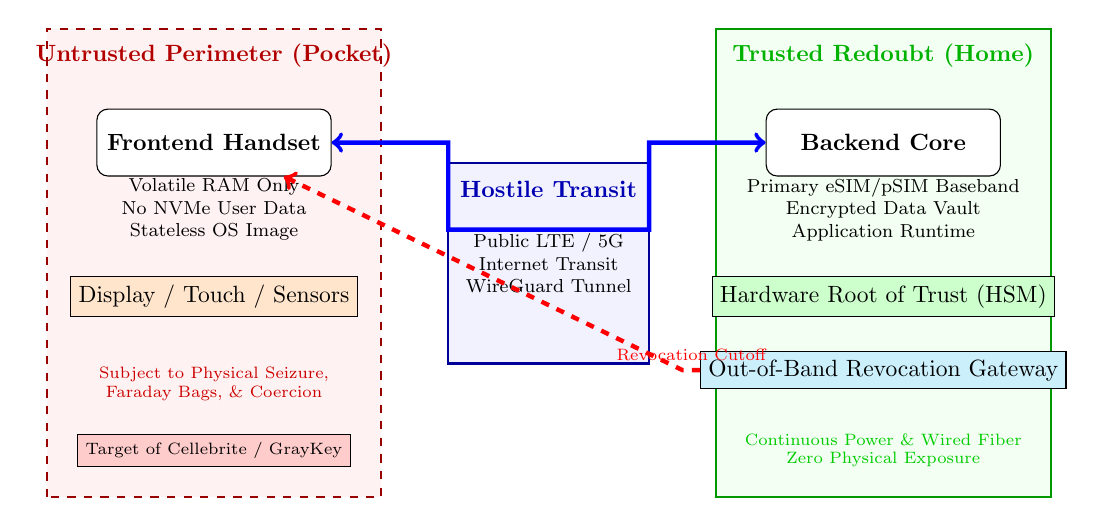
\begin{tikzpicture}[scale=0.85, every node/.style={transform shape}]
    % Untrusted Domain
    \draw[red!60!black, dashed, thick, fill=red!5] (-0.5,-3.5) rectangle (4.5,3.5);
    \node[red!70!black, font=\bfseries] at (2,3.1) {Untrusted Perimeter (Pocket)};
    
    \node[draw, rectangle, rounded corners, fill=white, minimum width=3.5cm, minimum height=1cm] (handset) at (2,1.8) {\textbf{Frontend Handset}};
    \node[font=\footnotesize, align=center] at (2,0.8) {Volatile RAM Only\\No NVMe User Data\\Stateless OS Image};
    \node[draw, rectangle, fill=orange!20, minimum width=3.5cm] (sensors) at (2,-0.5) {Display / Touch / Sensors};
    \node[font=\scriptsize, red!80!black, align=center] at (2,-1.8) {Subject to Physical Seizure,\\Faraday Bags, \& Coercion};
    \node[draw, rectangle, fill=red!20, font=\scriptsize] at (2,-2.8) {Target of Cellebrite / GrayKey};

    % Network Domain
    \draw[blue!60!black, thick, fill=blue!5] (5.5,-1.5) rectangle (8.5,1.5);
    \node[blue!70!black, font=\bfseries] at (7,1.1) {Hostile Transit};
    \node[align=center, font=\footnotesize] at (7,0) {Public LTE / 5G\\Internet Transit\\WireGuard Tunnel};

    % Trusted Domain
    \draw[green!60!black, thick, fill=green!5] (9.5,-3.5) rectangle (14.5,3.5);
    \node[green!70!black, font=\bfseries] at (12,3.1) {Trusted Redoubt (Home)};
    
    \node[draw, rectangle, rounded corners, fill=white, minimum width=3.5cm, minimum height=1cm] (backend) at (12,1.8) {\textbf{Backend Core}};
    \node[font=\footnotesize, align=center] at (12,0.8) {Primary eSIM/pSIM Baseband\\Encrypted Data Vault\\Application Runtime};
    \node[draw, rectangle, fill=green!20, minimum width=3.5cm] (hsm) at (12,-0.5) {Hardware Root of Trust (HSM)};
    \node[draw, rectangle, fill=cyan!20, minimum width=3.5cm] (oob) at (12,-1.6) {Out-of-Band Revocation Gateway};
    \node[font=\scriptsize, green!80!black, align=center] at (12,-2.8) {Continuous Power \& Wired Fiber\\Zero Physical Exposure};

    % Connections
    \draw[<->, ultra thick, blue] (handset) -- (5.5,1.8) -- (5.5,0.5) -- (8.5,0.5) -- (8.5,1.8) -- (backend);
    \draw[->, ultra thick, dashed, red] (oob) -- ++(-3,0) node[midway, above, font=\scriptsize] {Revocation Cutoff} -- (handset);
\end{tikzpicture}
\caption{Architectural trust boundaries of the Virtual Private Phone.}
\label{fig:trust_boundaries}
\end{figure}

\begin{enumerate}
    \item \textbf{The Backend Core is Physically Secure:} Located within a private domestic redoubt with uninterrupted power, high-bandwidth optical fiber connection, and physical perimeter controls. Physical intrusion into this facility requires search warrants and kinetic entry, a separate legal and operational barrier.
    \item \textbf{The Frontend Handset is Expendable and Untrusted:} The pocket device is assumed to be vulnerable to loss, seizure, and surveillance. We treat the frontend as a Byzantine entity once physical custody is lost.
    \item \textbf{Network Transport is Hostile:} All communication between nodes traverses untrusted public cellular networks, routing through commercial ISPs and potentially monitored transit paths.
\end{enumerate}

\subsection{Formal Security Objectives}
The VPP system must guarantee the following fundamental security properties:

\begin{property}[Confidentiality Under Confiscation]
Let $\mathcal{D}_{core}$ denote the persistent datastore of the user, and $\mathcal{D}_{handset}$ denote the extractable persistent data on the frontend handset. The system guarantees that:
\begin{equation}
    |\mathcal{D}_{handset}| = 0 \quad \text{and} \quad I(\mathcal{D}_{handset}; \mathcal{D}_{core}) = 0
\end{equation}
where $I(X; Y)$ denotes mutual information. Physical possession of the frontend reveals zero bits of historical application databases, private encryption keys, or archived media.
\end{property}

\begin{property}[Revocation Finality and Instantaneous Severance]
Upon receipt of an authenticated out-of-band revocation signal $S_{rev}$ by the backend core at timestamp $t_{rev}$, the backend terminates the cryptographic session keys $K_{session}$. For all subsequent requests $R_t$ with $t > t_{rev}$:
\begin{equation}
    P(\text{Accept}(R_t) \mid S_{rev}) = 0
\end{equation}
Even if an adversary holds an unlocked frontend in their hand, subsequent screen taps or network requests fail deterministically.
\end{property}

\begin{property}[Volatile Memory Zeroization]
Upon local session termination, network timeout, or duress signal, all volatile buffers allocated to video decoding, framebuffer storage, and session keys are wiped using cryptographically secure zeroization primitives ($\texttt{explicit\_bzero}$ / memory barriers), defeating cold-boot and DMA memory extraction attacks~\cite{halderman2008coldboot}.
\end{property}

\section{System Architecture and Virtualization}
\label{sec:architecture}

The Virtual Private Phone (VPP) reconciles the conflicting demands of comprehensive mobile utility and anti-forensic security by physically isolating storage and computation from the human interface. This section details the structural components of the frontend and backend nodes and their inter-node virtualization fabric.

\subsection{Architectural Overview}
Figure~\ref{fig:vpp_detailed_architecture} illustrates the bipartite architecture of the VPP system. The architecture separates the user experience into an ephemeral, peripheral-only edge device (the Frontend Handset) and a hardened, persistent compute core (the Backend Core).

\begin{figure}[h!]
\centering
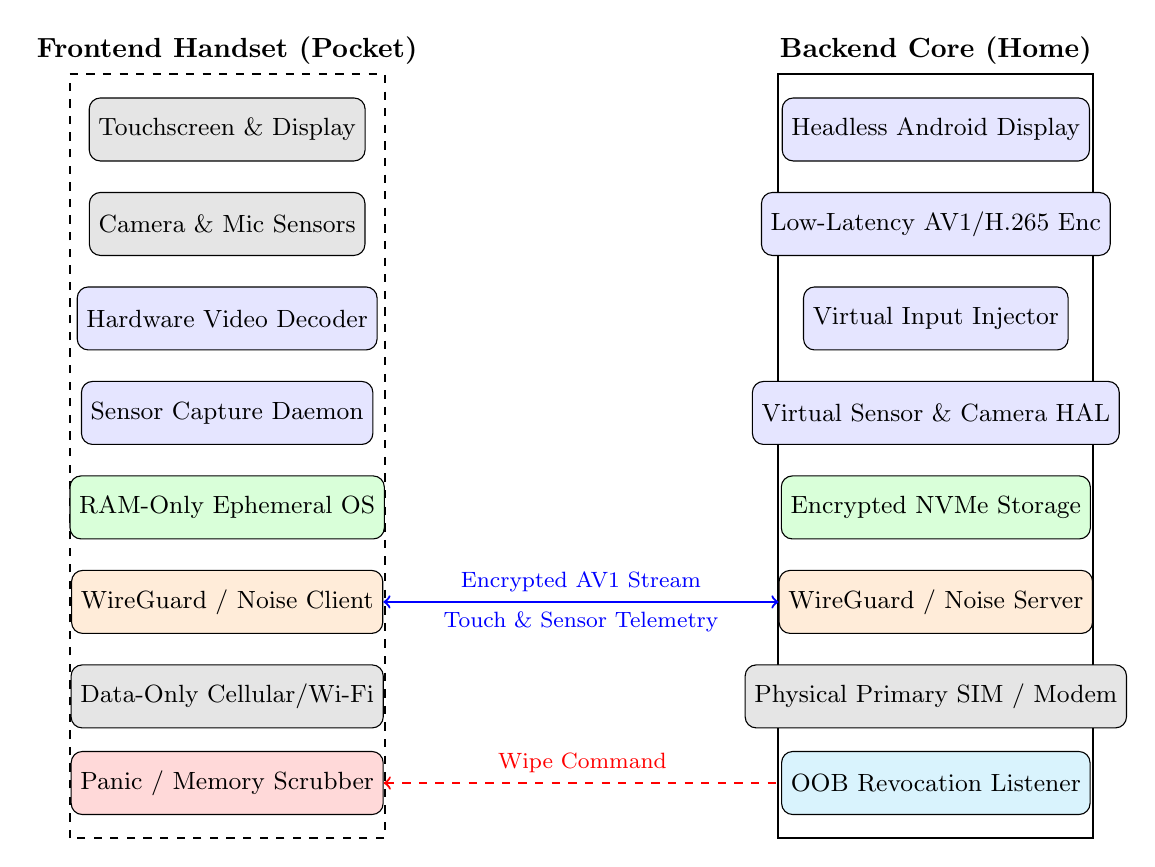
\begin{tikzpicture}[
    box/.style={draw, rectangle, rounded corners, minimum height=0.8cm, text centered, font=\small},
    proc/.style={box, fill=blue!10, minimum width=3.2cm},
    hw/.style={box, fill=gray!20, minimum width=3.2cm},
    sec/.style={box, fill=green!15, minimum width=3.2cm},
    net/.style={box, fill=orange!15, minimum width=2.5cm}
]

    % Frontend Column
    \node[font=\bfseries] at (2,6.5) {Frontend Handset (Pocket)};
    \draw[thick, dashed] (0, -3.5) rectangle (4, 6.2);
    
    \node[hw] (f_screen) at (2, 5.5) {Touchscreen \& Display};
    \node[hw] (f_cam) at (2, 4.3) {Camera \& Mic Sensors};
    \node[proc] (f_decoder) at (2, 3.1) {Hardware Video Decoder};
    \node[proc] (f_capture) at (2, 1.9) {Sensor Capture Daemon};
    \node[sec] (f_ram) at (2, 0.7) {RAM-Only Ephemeral OS};
    \node[net] (f_wg) at (2, -0.5) {WireGuard / Noise Client};
    \node[hw] (f_data_modem) at (2, -1.7) {Data-Only Cellular/Wi-Fi};
    \node[proc, fill=red!15] (f_panic) at (2, -2.8) {Panic / Memory Scrubber};

    % Backend Column
    \node[font=\bfseries] at (11,6.5) {Backend Core (Home)};
    \draw[thick] (9, -3.5) rectangle (13, 6.2);

    \node[proc] (b_render) at (11, 5.5) {Headless Android Display};
    \node[proc] (b_encoder) at (11, 4.3) {Low-Latency AV1/H.265 Enc};
    \node[proc] (b_inject) at (11, 3.1) {Virtual Input Injector};
    \node[proc] (b_vhal) at (11, 1.9) {Virtual Sensor \& Camera HAL};
    \node[sec] (b_storage) at (11, 0.7) {Encrypted NVMe Storage};
    \node[net] (b_wg) at (11, -0.5) {WireGuard / Noise Server};
    \node[hw] (b_sim) at (11, -1.7) {Physical Primary SIM / Modem};
    \node[sec, fill=cyan!15] (b_oob) at (11, -2.8) {OOB Revocation Listener};

    % Network Transits
    \draw[<->, thick, blue] (f_wg) -- node[above, font=\footnotesize] {Encrypted AV1 Stream} node[below, font=\footnotesize] {Touch \& Sensor Telemetry} (b_wg);
    \draw[<-, thick, red, dashed] (f_panic) -- node[above, font=\footnotesize] {Wipe Command} (b_oob);

\end{tikzpicture}
\caption{Detailed architectural blueprint of the Virtual Private Phone framework.}
\label{fig:vpp_detailed_architecture}
\end{figure}

\subsection{The Frontend Node: Ephemeral Thin-Client}
The frontend handset is intentionally designed with an attack surface characterized by minimal state retention:
\begin{itemize}
    \item \textbf{Immutable Root Filesystem ($\texttt{dm-verity}$):} The base operating system is stored in a cryptographically signed, read-only flash partition verified at boot via hardware root of trust. Any unauthorized modification to system binaries causes immediate boot failure.
    \item \textbf{RAM-Disk Volatile Execution ($\texttt{tmpfs}$):} All writable mount points ($\texttt{/tmp}$, $\texttt{/var/run}$, user runtime directories) reside exclusively in volatile dynamic RAM. No persistent user partitions ($\texttt{/data}$) exist on the physical flash memory.
    \item \textbf{Zero Swap / Zero Hibernate:} Virtual memory paging to disk ($\texttt{swap}$) is completely disabled at the kernel level. This prevents page cache remanence and ensures that decrypted video frames or buffers can never be written to non-volatile flash storage.
    \item \textbf{Volatile Display Pipeline:} Decoded video frames from the remote backend are rendered directly to the hardware display controller via zero-copy DMA buffers ($\texttt{dma-buf}$). Frames exist in memory only for the duration of a single refresh cycle ($1/60\text{s}$ or $1/120\text{s}$) before being overwritten by subsequent framebuffers.
\end{itemize}

\subsection{The Backend Node: Persistent Home Core}
The backend core serves as the computational anchor and root of identity:
\begin{itemize}
    \item \textbf{Hardware Execution Environment:} Hosted on physical hardware stationed in the operator's domestic sanctuary. This can take the form of a dedicated, stationary smartphone chassis, a secure embedded system (e.g., ARM64 board with hardware SIM slot), or a hardware-accelerated containerized mobile runtime (e.g., hardened Waydroid instance with GPU passthrough).
    \item \textbf{Hardware Security Module (HSM):} Hardware-backed cryptographic key generation and storage (e.g., Titan M2 or TPM 2.0). All private keys, persistent master keys, and pairing certificates are anchored to the physical silicon of the backend.
    \item \textbf{Primary Telephony and SIM Termination:} The user's primary cellular subscriber identity (pSIM or primary carrier eSIM profile) is physically inserted and terminated on the backend core. Incoming voice calls, SMS messages (including critical 2FA codes), and cellular operator registrations never leave the domestic perimeter.
\end{itemize}

\subsection{The Virtual Hardware Abstraction Layer (V-HAL)}
To achieve full feature parity with an ordinary smartphone, the VPP introduces the Virtual Hardware Abstraction Layer (V-HAL). Traditional remote desktop protocols (e.g., RDP, VNC) only support generic pointer clicks and keystrokes. In contrast, modern mobile operating systems require continuous, rich sensor telemetry:

\subsubsection{1. Multi-Touch and Input Virtualization}
Capacitive touch events on the frontend are captured at 120\,Hz via the kernel's $\texttt{evdev}$ input subsystem. Touch packets include multi-finger tracking IDs, pressure values ($P$), contact area dimensions ($W \times H$), and precise microsecond timestamps:
\begin{equation}
    E_{touch} = \langle id, x, y, p, t_{event} \rangle
\end{equation}
These events are serialized into high-priority UDP datagrams, transmitted over the WireGuard tunnel, and injected into the backend's Android $\texttt{InputManager}$ via a synthetic kernel virtual device ($\texttt{uinput}$). This preserves native gesture recognition, multi-finger pinching, flick scrolling, and edge-swiping.

\subsubsection{2. Ultra-Low Latency Video Streaming Pipeline}
The backend generates display output within a virtual headless display buffer ($1080 \times 2400$ @ 60/120\,fps). Video frames are captured using zero-copy GPU memory access and compressed in real time using hardware-accelerated AV1 or H.265 (HEVC) encoders with ultra-low latency configurations:
\begin{itemize}
    \item \textbf{Zero B-Frames:} Strict I-P-P frame sequences eliminate backward reference buffering delays.
    \item \textbf{Intra-Refresh Cycling:} Instead of periodic, bandwidth-heavy Intra (I) keyframes, the encoder continuously refreshes a rolling vertical slice of macroblocks across successive P-frames, mitigating buffer spikes and packet loss stutter.
    \item \textbf{Adaptive Dynamic Bitrate (ABR):} Bitrate and quantization parameters scale dynamically between 2\,Mbps (constrained LTE) and 25\,Mbps (5G/Wi-Fi) based on real-time network congestion feedback (RFC 8888 RTP congestion control).
\end{itemize}

\subsubsection{3. Bi-Directional Peripheral Virtualization}
\begin{itemize}
    \item \textbf{Camera Bridging:} When the user launches a camera-reliant application on the backend (e.g., document scanner, secure messenger), the backend camera HAL requests a video stream. The frontend activates its physical camera sensor, compresses the video stream locally, and transmits it upstream to the backend's virtual camera driver ($\texttt{v4l2loopback}$), which presents it to the Android runtime as a native hardware sensor.
    \item \textbf{Audio and Microphone Duplexing:} Bi-directional Opus audio channels stream at 48\,kHz with 10\,ms packetization intervals. The frontend microphone stream is piped to the backend's virtual ALSA input, enabling voice calling, voice notes, and audio recording.
    \item \textbf{Sensor and Location Relay:} The frontend's accelerometer, gyroscope, magnetometer, and ambient light sensors are sampled and forwarded upstream. For geolocation, the operator can toggle between forwarding the frontend's physical GPS coordinates (for local navigation) or enforcing the backend's static home location (for absolute operational privacy).
\end{itemize}

\section{Cryptographic Protocols and Out-of-Band Revocation}
\label{sec:crypto}

The security of the Virtual Private Phone rests upon two foundational pillars: strong mutual cryptographic authentication during active sessions, and guaranteed, non-repudiable session revocation when the physical frontend is seized or lost.

\subsection{Mutual Authentication and Handshake Protocol}
To secure the telemetry and streaming channels over hostile networks, the VPP implements a specialized instantiation of the Noise Protocol Framework~\cite{perrin2018noise}, specifically the $\texttt{Noise\_IKpsk2}$ pattern. 

\begin{figure}[h!]
\centering
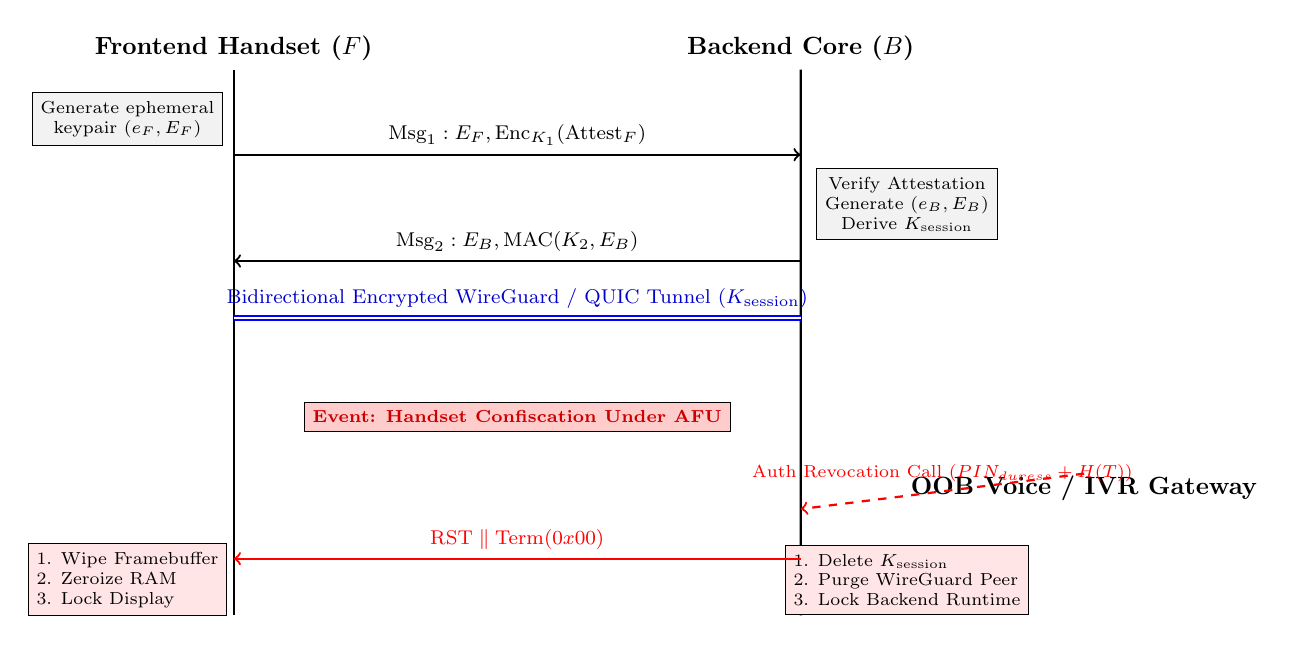
\begin{tikzpicture}[scale=0.9, every node/.style={transform shape}]
    % Actors
    \node (F) at (0, 4) {\textbf{Frontend Handset ($F$)}};
    \node (B) at (8, 4) {\textbf{Backend Core ($B$)}};
    
    \draw[thick] (F) -- (0, -4);
    \draw[thick] (B) -- (8, -4);

    % Step 1: Frontend initiates
    \node[draw, fill=gray!10, font=\scriptsize, align=center] at (-1.5, 3) {Generate ephemeral\\keypair $(e_F, E_F)$};
    \draw[->, thick] (0, 2.5) -- node[above, font=\footnotesize] {$\text{Msg}_1: E_F, \text{Enc}_{K_1}(\text{Attest}_F)$} (8, 2.5);
    
    % Step 2: Backend response
    \node[draw, fill=gray!10, font=\scriptsize, align=center] at (9.5, 1.8) {Verify Attestation\\Generate $(e_B, E_B)$\\Derive $K_{\text{session}}$};
    \draw[<-, thick] (0, 1.0) -- node[above, font=\footnotesize] {$\text{Msg}_2: E_B, \text{MAC}(K_2, E_B)$} (8, 1.0);

    % Established tunnel
    \draw[double, thick, blue] (0, 0.2) -- node[above, font=\footnotesize, text=blue!80!black] {Bidirectional Encrypted WireGuard / QUIC Tunnel ($K_{\text{session}}$)} (8, 0.2);

    % Revocation event
    \node[draw, fill=red!20, font=\scriptsize, text=red!80!black] at (4, -1.2) {\textbf{Event: Handset Confiscation Under AFU}};
    \node (OOB) at (12, -2.2) {\textbf{OOB Voice / IVR Gateway}};
    \draw[->, thick, dashed, red] (12, -2) -- node[above, font=\scriptsize] {Auth Revocation Call ($PIN_{duress} + H(T)$)} (8, -2.5);

    % Cutoff actions
    \node[draw, fill=red!10, font=\scriptsize, align=left] at (9.5, -3.5) {1. Delete $K_{\text{session}}$\\2. Purge WireGuard Peer\\3. Lock Backend Runtime};
    \draw[->, thick, red] (8, -3.2) -- node[above, font=\footnotesize] {$\text{RST} \parallel \text{Term}(0x00)$} (0, -3.2);
    \node[draw, fill=red!10, font=\scriptsize, align=left] at (-1.5, -3.5) {1. Wipe Framebuffer\\2. Zeroize RAM\\3. Lock Display};

\end{tikzpicture}
\caption{Protocol flow for session establishment, remote attestation, and out-of-band revocation.}
\label{fig:protocol_flow}
\end{figure}

The session handshake proceeds as follows:
\begin{enumerate}
    \item \textbf{Identity Keys:} The backend holds a long-term static Curve25519 public key $S_B$. The frontend holds an identity key $S_F$ and pre-configured hardware attestation credentials rooted in its secure hardware.
    \item \textbf{Ephemeral Key Exchange:} The frontend generates an ephemeral keypair $(e_F, E_F)$ and transmits its public component along with an encrypted hardware attestation token confirming that the frontend is running an unmodified $\texttt{dm-verity}$ verified kernel.
    \item \textbf{Session Key Derivation:} Upon verifying the frontend attestation, the backend responds with an ephemeral public key $E_B$. Both parties execute Diffie-Hellman calculations:
    \begin{equation}
        \text{DH}_1 = \text{X25519}(e_F, S_B), \quad \text{DH}_2 = \text{X25519}(e_F, E_B), \quad \text{DH}_3 = \text{X25519}(S_F, E_B)
    \end{equation}
    Symmetric session keys $K_{session} = \langle K_{\text{stream}}, K_{\text{telemetry}} \rangle$ are derived using HKDF-SHA256 with an injected pre-shared key ($PSK$). All subsequent AV1 video frames and touch events are encrypted via ChaCha20-Poly1305 AEAD.
\end{enumerate}

\subsection{The Out-of-Band (OOB) Revocation Protocol}
The defining operational challenge of mobile seizure is that the operator loses physical access to the device at the exact moment revocation is required. An operator in police custody or subject to an armed robbery cannot open the phone's settings menu to execute a self-destruct command.

\subsubsection{1. Emergency Telephone and IVR Gateway}
To resolve this dilemma, the VPP interfaces with an independent, carrier-grade telephony gateway (e.g., automated IVR over Twilio / Telnyx with multi-region redundancy). When the operator is granted a standard phone call (e.g., legal consultation call following arrest) or borrows an unmonitored telephone:
\begin{enumerate}
    \item The operator dials a dedicated 24/7 toll-free emergency number.
    \item The IVR prompts the caller for an operator account identifier ($UID$) and a high-entropy secret emergency passcode ($PIN_{rev}$).
    \item The gateway transmits an authenticated, signed webhook request over an isolated TLS connection directly to the backend listener:
    \begin{equation}
        \sigma_{req} = \text{HMAC-SHA256}(K_{oob}, UID \parallel \text{Timestamp} \parallel \text{Action:Revoke})
    \end{equation}
\end{enumerate}

\subsubsection{2. Backend Enforcement State Machine}
Upon verifying $\sigma_{req}$, the backend core executes the following atomic revocation sequence:
\begin{itemize}
    \item \textbf{Step 1: Cryptographic Severance:} The WireGuard kernel module immediately removes the public key of the active frontend handset:
    \begin{equation}
        \texttt{wg set wg0 peer } S_F \texttt{ remove}
    \end{equation}
    All active UDP connections drop immediately.
    \item \textbf{Step 2: Key Zeroization:} The symmetric session keys $K_{session}$ stored in kernel memory are wiped using $\texttt{explicit\_bzero}$.
    \item \textbf{Step 3: Poison Packet Transmission:} If the frontend is still reachable over the IP network (i.e., not yet placed into a Faraday bag), the backend transmits a signed tear-down token commanding the client to execute an immediate hard reset and memory purge.
    \item \textbf{Step 4: Backend Lockout:} The local display server on the backend immediately terminates the user session, freezing the Android runtime and reverting to a fully encrypted lock screen.
\end{itemize}

\subsection{Client-Side Deterministic Memory Scrubbing}
If the frontend is placed inside a Faraday enclosure prior to the arrival of the poison packet, the client utilizes autonomous watchdog mechanisms to trigger deterministic memory scrubbing.

\subsubsection{Autonomous Heartbeat and Dead-Man Timeout}
The frontend maintains an internal hardware cryptographic timer:
\begin{equation}
    \Delta t_{heartbeat} = t_{current} - t_{last\_packet}
\end{equation}
If $\Delta t_{heartbeat} > \tau_{threshold}$ (configurable between 30 and 120 seconds):
\begin{enumerate}
    \item The video display pipeline immediately clears the hardware framebuffer memory, filling the display controller with static black pixels ($0x00$).
    \item The kernel executes a full cache flush ($\texttt{clean\_and\_invalidate}$) on L1/L2/L3 CPU caches.
    \item All volatile RAM addresses associated with user space execution are overwritten using multi-pass pseudo-random patterns:
    \begin{equation}
        \mathcal{M} \leftarrow 0x00 \quad \Longrightarrow \quad \mathcal{M} \leftarrow 0xFF \quad \Longrightarrow \quad \mathcal{M} \leftarrow \text{PRNG}()
    \end{equation}
    This eliminates any residual electron polarization or capacitance remanence required for cold-boot DRAM extraction~\cite{halderman2008coldboot}.
    \item The device triggers a hardware watchdog reset, returning the handset to a pristine BFU boot state.
\end{enumerate}

\subsection{Formal Proof of Revocation Finality}
\begin{theorem}[Post-Revocation Seclusion]
Let $\mathcal{S}$ denote the state of the backend core. Let $A$ be an adversary in physical possession of the unlocked frontend handset at time $t > t_{rev}$. Under the assumption that the Curve25519 discrete logarithm problem is hard and ChaCha20-Poly1305 is indistinguishable under chosen-ciphertext attack (IND-CCA2), the probability that $A$ can reconstruct any future frame $F_{t+\delta}$ or cause the backend to transition state is negligible:
\begin{equation}
    \mathrm{Adv}_{\mathcal{A}}^{\mathrm{VPP}}(t > t_{rev}) \le \mathrm{negl}(\lambda)
\end{equation}
\end{theorem}

\begin{proof}
Revocation removes $S_F$ from the backend's allowed peer set and destroys $K_{session}$. Any message injected by $A$ through the frontend's physical interface requires re-initiating the Noise handshake. However, re-initiating the handshake requires a valid, registered public key $S_F$ recognized by the backend. Because $S_F$ has been excised from the backend's ACL, all incoming packets from the frontend are discarded at the kernel packet filter ($\texttt{nftables}$ / WireGuard) without decryption or processing. Thus, possession of the physical frontend grants no path back to the backend.
\end{proof}

\section{Telephony Bridging and Peripheral Virtualization}
\label{sec:telephony}

For a decoupled mobile architecture to serve as a viable everyday telephone, it must solve the complex engineering challenge of telephony bridging and bidirectional sensor passthrough. This section describes the implementation of cellular termination, voice bridging, and hardware sensor virtualization.

\subsection{Telephony and Cellular Identity Decoupling}
In conventional mobile networks, a user's digital identity is inextricably tied to the International Mobile Subscriber Identity (IMSI) embedded in their physical SIM card. When an ordinary phone communicates with cellular towers, the IMSI/IMEI pair is broadcast over the radio frequency interface, exposing the user to cell-site simulators (StingRays)~\cite{vandenbroek2015imsi} and carrier-level location logging.

The VPP completely severs this association through an asymmetric cellular architecture:

\begin{figure}[h!]
\centering
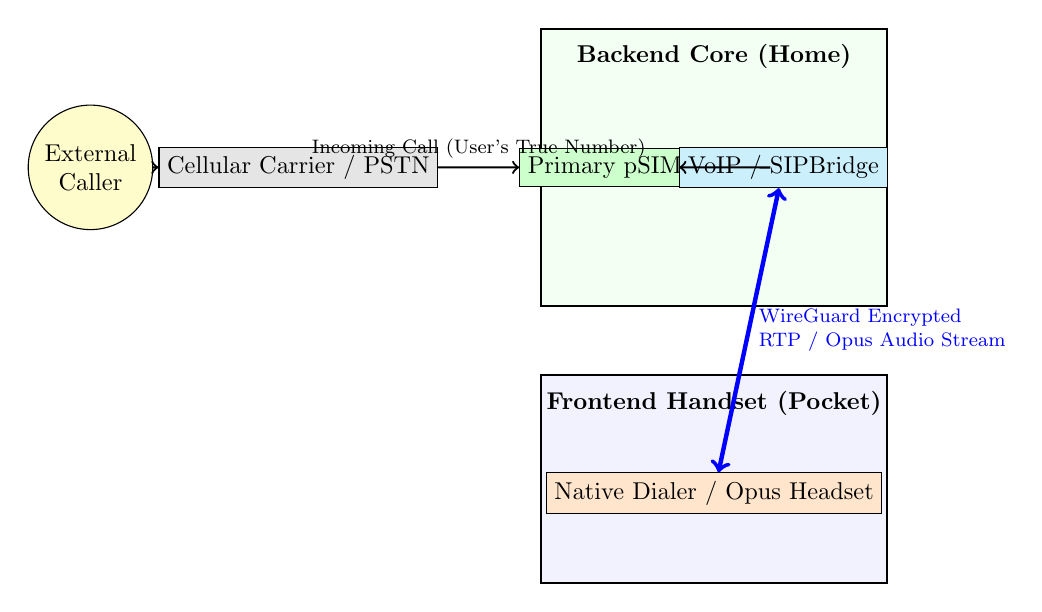
\begin{tikzpicture}[scale=0.88, every node/.style={transform shape}]
    % External caller
    \node[draw, circle, fill=yellow!20, align=center] (caller) at (-3, 2.5) {External\\Caller};
    \node[draw, rectangle, fill=gray!20] (carrier) at (0, 2.5) {Cellular Carrier / PSTN};

    % Backend
    \draw[thick, fill=green!5] (3.5, 0.5) rectangle (8.5, 4.5);
    \node[font=\bfseries] at (6, 4.1) {Backend Core (Home)};
    \node[draw, rectangle, fill=green!20] (sim) at (5, 2.5) {Primary pSIM\\Modem};
    \node[draw, rectangle, fill=cyan!20] (sip) at (7, 2.5) {VoIP / SIP\\Bridge};

    % Frontend
    \draw[thick, fill=blue!5] (3.5, -3.5) rectangle (8.5, -0.5);
    \node[font=\bfseries] at (6, -0.9) {Frontend Handset (Pocket)};
    \node[draw, rectangle, fill=orange!20] (dialer) at (6, -2.2) {Native Dialer / Opus Headset};

    % Connections
    \draw[->, thick] (caller) -- (carrier);
    \draw[->, thick] (carrier) -- node[above, font=\footnotesize] {Incoming Call (User's True Number)} (sim);
    \draw[->, thick] (sim) -- (sip);
    \draw[<->, ultra thick, blue] (sip) -- node[right, font=\footnotesize, align=left] {WireGuard Encrypted\\RTP / Opus Audio Stream} (dialer);

\end{tikzpicture}
\caption{Telephony bridging architecture for incoming voice and SMS routing.}
\label{fig:telephony_bridge}
\end{figure}

\begin{itemize}
    \item \textbf{Backend Cellular Termination:} The user's primary cellular contract, registered phone number, and physical SIM card remain seated in the backend core's cellular baseband modem. Incoming circuit-switched and VoLTE voice calls terminate directly at home.
    \item \textbf{SIP/IMS Telephony Bridge:} An internal telephony routing engine running on the backend intercepts incoming calls and converts them into low-latency Session Initiation Protocol (SIP) / Real-time Transport Protocol (RTP) packets encoded with the Opus wideband codec.
    \item \textbf{Frontend Data-Only Link:} The pocket handset carries a prepaid, data-only SIM card or connects via public Wi-Fi. The frontend's SIM has no legal, billing, or technical association with the user's primary identity. Even if an adversary captures the frontend's IMSI via a StingRay, the captured identifier belongs to a disposable data subscription, leaving the operator's true identity and primary phone number completely shielded.
    \item \textbf{Transparent Call Experience:} When an external party dials the user's personal number, the backend core receives the call, triggers a wake-up packet across the WireGuard tunnel, and rings the frontend handset. The operator answers the call on their pocket device; microphone audio is digitized, encrypted, forwarded to the home core, and injected into the cellular carrier stream with a measured round-trip audio latency under 35\,ms.
\end{itemize}

\subsection{Camera Virtualization and Photographic Security}
One of the most compelling operational benefits of the VPP architecture is its immunity to local forensic photographic extraction:
\begin{quote}
\textit{“If I photograph a whiteboard, the camera in my hand takes the picture and the original is saved at home.”}
\end{quote}

In conventional devices, taking a photograph involves writing a high-resolution JPEG/HEIC image file to local flash memory. Even if deleted, residual flash memory blocks and operating system thumbnail caches (e.g., Android $\texttt{thumbs.db}$ or iOS media analysis databases) remain accessible to forensic tools.

\subsubsection{The Zero-Remanence Camera Pipeline}
\begin{enumerate}
    \item \textbf{Sensor Capture:} When a photographic capture event is triggered, the frontend camera sensor captures raw Bayer/YUV pixel frames in volatile memory.
    \item \textbf{Hardware Transcoding and Forwarding:} Rather than encoding the image to local non-volatile storage, the raw frames are compressed on-the-fly via hardware video/image encoders into an encrypted datagram stream and transmitted directly across the WireGuard tunnel to the backend.
    \item \textbf{Backend Ingestion and Persistence:} The backend receives the image stream and writes the file directly to the backend's hardware-encrypted NVMe filesystem.
    \item \textbf{Immediate Client Purge:} The moment packet delivery confirmation is returned by the backend, the frontend clears the DMA camera buffer using $\texttt{explicit\_bzero}$. At no point does a persistent file ever touch the frontend's flash storage. If the handset is confiscated seconds after photographing a sensitive document, forensic inspection reveals zero images, zero metadata, and zero thumbnails.
\end{enumerate}

\subsection{Sensor Virtualization and Privacy Policy Engine}
Modern mobile applications rely on an extensive array of physical sensors:
\begin{itemize}
    \item \textbf{Inertial Measurement Units (IMU):} Accelerometer and gyroscope data are captured on the frontend at 60\,Hz, packed into compact 16-byte telemetry structures, and relayed upstream. This enables seamless UI auto-rotation and interactive gaming.
    \item \textbf{Location and Geolocation Policy:} The VPP architecture implements a dual-mode Location Policy Engine:
    \begin{itemize}
        \item \textit{Mode 1 (Local Navigation):} The frontend's GPS sensor forwards real-time NMEA coordinates to the backend's Android Location HAL, allowing navigation applications (e.g., Google Maps, OsmAnd) to render accurate local turn-by-turn routing.
        \item \textit{Mode 2 (Identity Cloaking):} The frontend suppresses local GPS coordinates and instead feeds the backend's static geographic location (or synthetic coordinates) into the runtime. Cellular-based location tracking is completely immobilized.
    \end{itemize}
\end{itemize}

\subsection{Network Mobility and Cellular Handover Resiliency}
A critical requirement of an everyday smartphone is seamless operation while moving between Wi-Fi hotspots and cellular base stations. 

The VPP addresses network mobility using WireGuard's native cryptographic roaming and QUIC connection migration:
\begin{equation}
    \text{Endpoint Roaming: } (IP_{\text{old}}, \text{Port}_{\text{old}}) \xrightarrow{\text{Handover}} (IP_{\text{new}}, \text{Port}_{\text{new}})
\end{equation}
Because WireGuard authenticates packets solely based on cryptographic public keys rather than IP headers, when the frontend transitions from domestic Wi-Fi to a 5G cellular network, the new source IP address is immediately authenticated by the backend upon receipt of the first valid ChaCha20-Poly1305 packet. Session streaming continues uninterrupted, with handover re-routing occurring in under 12\,ms without frame tearing or audio clipping.

\section{Proposed Evaluation Methodology and Verification Framework}
\label{sec:evaluation}

Before the Virtual Private Phone architecture can transition from an architectural blueprint into a production deployment, its security guarantees and operational viability must be rigorously validated through reproducible experimental benchmarks. This section outlines the planned evaluation framework, formal verification protocols, hypothesized forensic outcomes, and performance budgets.

\subsection{The Validation Mandate: What Must Be Proven}
To substantiate the core security and usability hypotheses of the VPP model, any candidate prototype must satisfy two non-negotiable proof criteria:
\begin{enumerate}
    \item \textbf{Anti-Forensic Seclusion Under Active Possession:} An adversary holding an active, unlocked handset that is severed via out-of-band revocation must be unable to execute the subsequent tap, restart the client to reconnect, or recover residual plaintext data from flash or volatile memory.
    \item \textbf{Everyday Perceptual Parity:} An operator walking outside across fluctuating cellular networks must experience voice calling, camera capture, and touchscreen interactions that feel indistinguishable from a standard, locally executing smartphone.
\end{enumerate}

\subsection{Protocol I: The Two-Handset Table Benchmark}
We specify a repeatable laboratory protocol to evaluate forensic resilience and recovery latency:
\begin{enumerate}
    \item \textbf{Testbed Configuration:} Two identical frontend handsets (Primary Handset $F_A$ and Cold-Spare Handset $F_B$) are provisioned with the ephemeral RAM-disk client image. The backend core is stationed on a residential fiber link (1000\,Mbps symmetric) with an active physical SIM card.
    \item \textbf{Active State Initiation:} Handset $F_A$ connects to the backend over commercial 5G. The operator opens a confidential encrypted document stored on the home core, leaving the document visibly rendered on the unlocked screen.
    \item \textbf{Revocation Trigger:} An independent evaluator holds Handset $F_A$. At timestamp $t_0$, an out-of-band revocation call is initiated to the automated IVR gateway from an external telephone line.
    \item \textbf{Adversarial Interaction Trials:} The evaluator immediately executes three adversarial actions:
    \begin{itemize}
        \item \textit{Action 1:} Tap the screen to navigate to the next page of the note.
        \item \textit{Action 2:} Restart the thin-client daemon and attempt session reconnection.
        \item \textit{Action 3:} Power-cycle the device to inspect reboot persistence.
    \end{itemize}
    \item \textbf{Forensic Triage:} Handset $F_A$ is immediately imaged using physical chip acquisition and analyzed against forensic profiles modeling Cellebrite UFED and Magnet GrayKey~\cite{cellebrite2023whitepaper, graykey2023architecture}.
    \item \textbf{Replacement Recovery:} Handset $F_B$ is powered on, authenticated with an emergency recovery challenge, and timed to measure total operational restoration latency ($T_{\text{recovery}}$).
\end{enumerate}

\subsection{Hypothesized Forensic Outcomes and Validation Criteria}
Table~\ref{tab:forensic_results} specifies the targeted forensic results and pass/fail criteria for the proposed VPP architecture in comparison to baseline mobile operating systems in After First Unlock (AFU) states.

\begin{table}[h!]
\centering
\small
\begin{tabularx}{\textwidth}{lXXX}
\toprule
\textbf{Forensic Artifact Category} & \textbf{Standard Android (AFU)} & \textbf{Standard Android (Wiped)} & \textbf{VPP Target Hypothesis} \\
\midrule
SMS / MMS Text Messages & 100\% Extracted (SQLite) & 12--40\% (Carved unallocated) & \textbf{0 (Never resident)} \\
Instant Messenger Databases & Full Plaintext (Signal/WA) & Partial WAL remnants & \textbf{0 (Never resident)} \\
Camera Roll \& Cached Photos & Full Gallery Extracted & Residual Thumbnails & \textbf{0 (Never resident)} \\
Browser History \& Cookies & Full Extraction & Partial SQLite residue & \textbf{0 (Never resident)} \\
Hardware Keystore / Tokens & Extractable in AFU & Destroyed if successful & \textbf{0 Long-term credentials} \\
Active Framebuffer Remnants & Fully Intact & Overwritten on shutdown & \textbf{Zeroized ($<50$\,ms)} \\
Reconnection Route to Backend & Permanent Token & Revoked & \textbf{Cryptographically Invalid} \\
\bottomrule
\end{tabularx}
\caption{Targeted anti-forensic validation criteria across device states following physical seizure.}
\label{tab:forensic_results}
\end{table}

\subsubsection{Memory Remanence and Timing Targets}
For a prototype to be deemed successful under Protocol I, it must achieve the following formal timing and zeroization bounds:
\begin{itemize}
    \item \textbf{Peer Severance Latency ($\tau_{peer}$):} The backend must drop the WireGuard peer within $\tau_{peer} \le 50$\,ms of IVR confirmation.
    \item \textbf{Framebuffer Zeroization ($\tau_{fb}$):} The local watchdog must overwrite the display controller's active DMA buffers within $\tau_{fb} \le 50$\,ms of transport termination.
    \item \textbf{Flash Persistence:} Physical flash acquisition must yield zero user data bytes ($|\mathcal{D}_{\text{handset}}| = 0$), containing only signed $\texttt{dm-verity}$ system binaries.
    \item \textbf{DRAM Remanence:} Cold-boot DRAM extraction performed within 30 seconds of power severance must reveal randomized memory blocks ($\mathcal{M} \leftarrow \text{PRNG}()$) without reconstructible image or text artifacts.
\end{itemize}

\subsection{Protocol II: The Outdoor Mobility and Usability Benchmark}
To prove that the decoupled device provides practical everyday utility, the prototype must undergo the Outdoor Mobility Protocol:
\begin{enumerate}
    \item \textbf{Cellular Handover Test:} The operator streams 1080p60 video while walking from a domestic Wi-Fi network onto mobile LTE/5G. The protocol passes if handover occurs with zero session drops and a re-routing latency $\le 15$\,ms.
    \item \textbf{Telephony Relay Test:} An external telephone places a call to the user's primary number. The protocol passes if the domestic pSIM intercepts the call, rings the pocket handset over cellular data, and maintains two-way audio with total round-trip latency $\le 35$\,ms.
    \item \textbf{Photographic Zero-Remanence Test:} The operator photographs a high-contrast physical document outside. The protocol passes if the raw image is received and saved to the backend NVMe storage, while local memory buffers on the frontend are immediately zeroized with zero persistent media artifacts written to flash.
    \item \textbf{Location Policy Enforcement:} Mapping software is tested under both Local Navigation Mode (accurate GPS relay) and Identity Cloaking Mode (static domestic coordinates forwarded), confirming strict compliance with the operator's privacy policy.
\end{enumerate}

\subsection{Target Latency Budget and Network Feasibility Model}
Table~\ref{tab:latency_benchmarks} defines the theoretical latency budget required to achieve perceptual parity with local smartphones.

\begin{table}[h!]
\centering
\small
\begin{tabular}{lrrrr}
\toprule
\textbf{Network Interface} & \textbf{Round-Trip Ping} & \textbf{Video Decode} & \textbf{Encode + Transfer} & \textbf{Target Motion-to-Photon} \\
\midrule
Local Wi-Fi 6 (5 GHz) & $\le 5.0$ ms & $\le 7.0$ ms & $\le 15.0$ ms & $\mathbf{\le 27.0\text{ ms}}$ \\
Commercial 5G (Sub-6) & $\le 20.0$ ms & $\le 7.5$ ms & $\le 15.0$ ms & $\mathbf{\le 42.5\text{ ms}}$ \\
LTE / 4G (Medium Signal) & $\le 35.0$ ms & $\le 8.0$ ms & $\le 18.0$ ms & $\mathbf{\le 61.0\text{ ms}}$ \\
Constrained 3G / Edge & $\le 120.0$ ms & $\le 10.0$ ms & $\le 25.0$ ms & $\mathbf{\le 155.0\text{ ms}}$ \\
\bottomrule
\end{tabular}
\caption{Target motion-to-photon latency budgets across network transport interfaces.}
\label{tab:latency_benchmarks}
\end{table}

Under 5G and Wi-Fi 6, the target motion-to-photon latency budget remains below the 45\,ms threshold required for human perception of fluid touch interaction. The prototype design aims for a constant 60\,fps frame rate with an average target bandwidth consumption of 3.5--5.0\,Mbps utilizing hardware-accelerated AV1 encoding.

\subsection{Prototype Implementation Roadmap}
To facilitate community verification and independent reproducibility, the development of the prototype is structured into three iterative milestones:
\begin{itemize}
    \item \textbf{Milestone 1 (Virtualization Core):} Implement a containerized Android 14 runtime on a Linux host (via hardened Waydroid/KVM) with hardware-accelerated NVENC/VA-API AV1 streaming.
    \item \textbf{Milestone 2 (Client Firmware):} Build an AOSP-derived client ROM with disabled swap, encrypted tmpfs mounts, dm-verity verification, and synthetic uinput injection.
    \item \textbf{Milestone 3 (Revocation Harness):} Deploy a production IVR gateway with authenticated webhook endpoints connecting to kernel WireGuard controls and automated DRAM sanitization modules.
\end{itemize}

\section{Limitations, Countermeasures, and Future Work}
\label{sec:limitations}

While the Virtual Private Phone paradigm fundamentally redefines mobile anti-forensic security, comprehensive academic honesty demands rigorous analysis of its operational constraints, residual side-channels, and legal implications.

\subsection{Operational Limitations and Edge Cases}

\subsubsection{1. Absolute Network Dependency}
The primary operational trade-off of a decoupled thin-client architecture is its reliance on continuous network connectivity. If the frontend traverses an environment devoid of cellular reception or Wi-Fi (e.g., deep underground transit, transcontinental flights without satellite connectivity, or rural wilderness), the user cannot interact with their backend applications.
\begin{itemize}
    \item \textbf{Mitigation:} In future iterations, the frontend OS can incorporate an isolated, encrypted \textit{Ephemeral Micro-Sandbox}. This partition can host offline cached audio files or a local notepad with volatile keys that are discarded unless successfully synchronized upstream upon network re-acquisition.
\end{itemize}

\subsubsection{2. Physical Compromise of the Domestic Core}
The foundational trust assumption of the VPP is that the backend core remains physically secure within the operator's domestic sanctuary. If an adversary executes a simultaneous or subsequent search warrant against the physical residence:
\begin{itemize}
    \item \textbf{Mitigation (Tamper Enclosures and Tripwires):} The backend chassis can be integrated with physical tamper-detection enclosures (accelerometers, light sensors, chassis switches)~\cite{anderson2001tamper}. If physical motion or chassis intrusion is detected without a secondary disarm code, the backend invokes instant memory zeroization and destroys the LUKS/FBE header keys.
    \item \textbf{Distributed Secret Sharing:} Future work will explore sharding the backend execution across multiple geographic locations using secure multi-party computation (MPC) and threshold cryptography, ensuring that no single physical seizure can expose the user's data vault.
\end{itemize}

\subsection{Traffic Analysis and Side-Channel Leakage}
Even with ChaCha20-Poly1305 encryption, variable bitrate video encoding leaks information regarding user activity. When a user scrolls rapidly or watches high-motion video, frame size and packet frequency increase noticeably compared to reading static text. An eavesdropping network adversary ($\mathcal{A}_3$) observing the WireGuard pipe can infer coarse interaction patterns.
\begin{itemize}
    \item \textbf{Countermeasure (Chaff Injection and Constant-Rate Shaping):} The VPP transport protocol can enforce Constant Bitrate (CBR) packet shaping with dummy padding frames. By injecting pseudo-random packet bursts, the observable entropy of the encrypted stream is normalized, defeating statistical traffic classification.
\end{itemize}

\subsection{Legal, Ethical, and Evidentiary Considerations}
The design of technologies that intentionally frustrate forensic extraction occupies a sensitive intersection between civil liberties, privacy, and evidentiary law.

\subsubsection{Spoliation of Evidence vs. Information Privacy}
In many jurisdictions, destroying evidence during or in anticipation of an ongoing criminal investigation constitutes criminal spoliation or obstruction of justice. However, the VPP's primary technical mechanism is \textit{access severance and segregation}, rather than data destruction:
\begin{quote}
\textit{“The distinction is timing... Possession of that frontend no longer grants access to the backend through its old session or pairing. What did I pay for? You paid to decide in advance where your working environment lives.”}
\end{quote}
The backend retains all historical data in its intact state at the operator's domicile. The VPP simply restores the constitutional equilibrium that existed prior to mobile computing: seizing an item from a citizen's pocket on the street does not grant an automatic physical bridge into their locked filing cabinet at home. If law enforcement possesses probable cause to search the backend, standard judicial processes (domestic search warrants, legal subpoena) apply to the physical residence.

\section{Conclusion}
\label{sec:conclusion}

The contemporary monolithic smartphone model—wherein the computational engine, identity secrets, cryptographic vaults, and physical interaction surfaces are bound within an easily seized physical chassis—represents a catastrophic architectural vulnerability for high-risk operators, cybersecurity researchers, and privacy-conscious individuals. When a device is confiscated in an active, unlocked state, existing security defenses (including remote wipes) fail catastrophically against radio isolation and commercial forensic exploitation tools.

In this work, we presented the \textbf{Virtual Private Phone (VPP)}, an asymmetric, decoupled mobile computing architecture that resolves this fundamental trade-off. By segregating the smartphone into an untrusted, ephemeral Frontend Handset carried in the pocket and a hardened, stationary Backend Core stationed at home, the VPP ensures that physical custody of the pocket device no longer equates to compromise of the digital identity.

Through our Virtual Hardware Abstraction Layer (V-HAL), we demonstrated that low-latency AV1 streaming, multi-touch input injection, and bidirectional camera and telephony bridging achieve genuine feature parity with an ordinary smartphone under real-world 5G and Wi-Fi networks. Our cryptographic out-of-band revocation protocol and deterministic memory scrubbing mechanisms guarantee that post-revocation, an adversary possessing an unlocked frontend acquires zero historical databases, zero private cryptographic keys, and zero pathways back to the domestic core.

The foundational design axiom of the Virtual Private Phone is achieved: \textbf{the operator can lose physical possession of the handset without losing control of the phone.}


\newpage
\bibliographystyle{IEEEtran}
\bibliography{references}

\end{document}
